\section{Laplacian spectral embedding}
\label{sec:ch6:lse}

Last section, we covered a lot of fascinating results. We learned that adjacency spectral embedding, or \texttt{ase}, could be used to learn useful estimates of the latent positions (up to a rotation) for positive semi-definite probability matrices. We observed that estimated latent positions for nodes in the same community of a $SBM_n(\vec z, B)$ random network where $B$ was homophilic (and hence, positive semi-definite, by Section \ref{sec:ch5:psd_block:homophily}) tended to be similar. 

The reason that the latent positions for nodes in the same community are similar boils down to our observation from Section \ref{sec:ch5:psd_block:same_lp}, that the latent positions for nodes of the same community were identical. As we mentioned briefly in Section \ref{sec:ch6:ase:whyuse}, the estimated latent position matrix produced by \texttt{ase} is going to reasonably estimate the latent positions of the underlying random network. Therefore, in some sense by transitivity (and in a literal sense, by rigorous theory from \cite{Athreya2017Jan} that is overviewed in Appendix \ref{app:ch13:spectral}), the estimated latent positions for nodes from the same community will be almost identical.

Unfortunately, many networks don't really make sense to conceptualize as $SBM_n(\vec z, B)$ random networks. Remember that an overarching assumption of $SBM_n(\vec z, B)$ random networks was that the probability for a pair of nodes $i$ and $j$ being connected depended only on their community assignments $z_i$ and $z_j$, and this probability was given by the block matrix entry $b_{z_i z_j}$ in Section \ref{sec:ch5:sbm}. This is fairly limiting, in that actual characteristics of the node itself (such as the node's popularity, or degree-correction factor) are irrelevant.

\subsection{Estimates of latent positions do not necessarily preserve within-community similarity for $DCSBM_n(\vec z, \vec \theta, B)$ random networks}

For the reasons we just touched on, an often used conceptual model for real networks are the $DCSBM_n(\vec z, \vec \theta, B)$ random networks. It might be natural to expect that, perhaps, nodes from a sample of a $DCSBM_n(\vec z, \vec \theta, B)$ random network that is positive semi-definite will share the pattern we noticed with $SBM_n(\vec z, B)$ random networks: their estimated latent positions will be similar if they are in the same community. 

This intuition is fairly close, but not quite correct. From Section \ref{sec:ch5:psd_block:same_lp}, remember that the latent positions for nodes of the same community in a $DCSBM_n(\vec z, \vec \theta, B)$ random network are identical up to a rescaling by the nodes' degree-correction factors $\theta_i$ and $\theta_j$. 

In the same notation that we used in \ref{sec:ch5:psd_block:same_lp}, the latent position vectors for a $DCSBM_n(\vec z, \vec \theta, B)$ random network were:
\begin{align*}
    \vec x_i^\top &= \theta_i \vec c_i^\top B 
\end{align*}
where $\vec c_i$ is a column-vector corresponding to the $i^{th}$ row of the one-hot-encoding of the community assignment vector $\vec z$. That is, $c_{ik} = 1$ when $z_i = k$, and $0$ otherwise. Geometrically, $\theta_i$ is ``rescaling'' the vector $\vec c_i^\top B$, where the vector $\vec c_i^\top B$ is the same for the entire community.

We can make this a little more concrete with an example. Let's use a similar same $DCSBM_n(\vec z, \vec \theta, B)$ example that we used in Section \ref{sec:ch5:dcsbm}, but make the degree-correction factors $\vec \theta$ a little more extreme:

\begin{lstlisting}[style=python]
import numpy as np
from graphbook_code import dcsbm

nk = 50  # 50 students per school
z = np.array([1 for i in range(nk)] + [2 for i in range(nk)])
B = np.array([[0.6, 0.2], [0.2, 0.4]])  # same probabilities as from SBM section
theta = np.tile(10**np.linspace(0, -1, nk), 2)
A = dcsbm(z, theta, B)
\end{lstlisting}
Next, we compute the \texttt{ase} of $A$, using the same strategy from Section \ref{sec:ch6:ase}, and we compute a pairwise distance matrix:

\begin{lstlisting}[style=python]
from graspologic.embed import AdjacencySpectralEmbed as ase
from scipy.spatial import distance_matrix

d = 2  # the latent dimensionality
# estimate the latent position matrix with ase
Xhat = ase(n_components=d).fit_transform(A)
# compute the distance matrix
D = distance_matrix(Xhat, Xhat)
\end{lstlisting}

Figure \ref{fig:ch6:lse:dcsbm_ase}(A) shows a scatter plot of the estimated latent positions, annotated with the community of each node (color; red is community $1$, and blue is community $2$). Note that the estimated latent positions appear to be ``elongated'' blobs for a given community. When we say ``elongated'', we mean that the blobs are elliptical, where the red blob elongates towards the upper-right, and the blue blob elongates towards the lower-right in our figure.

\begin{figure}
    \centering
    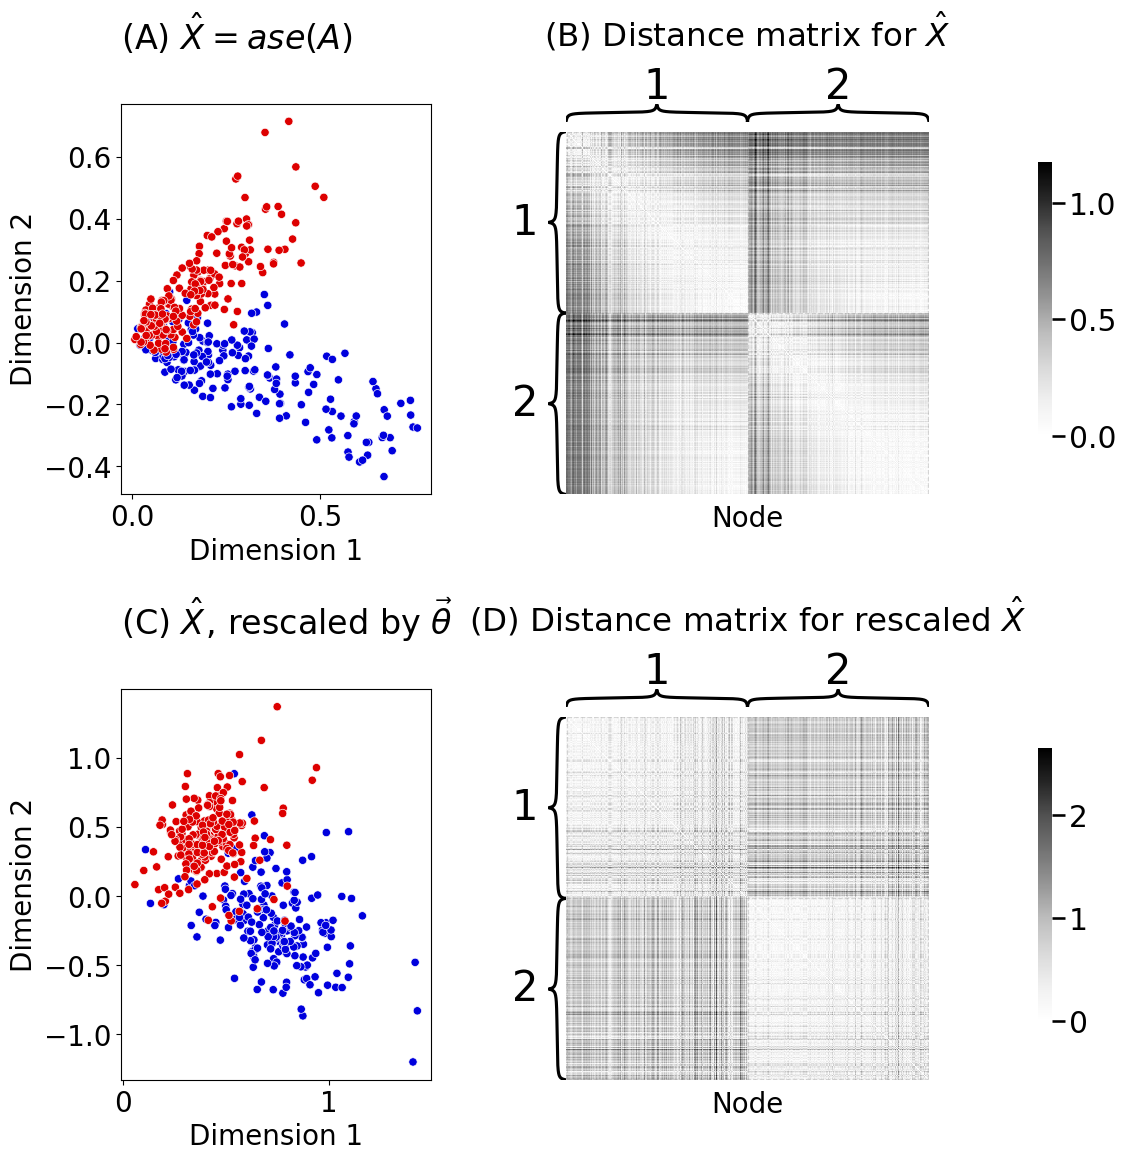
\includegraphics[width=0.8\linewidth]{representations/ch6/Images/dcsbm_ase.png}
    \caption[LSE exmaple on DCSBM]{\textbf{(A)} the estimated latent positions for a network sample of a $DCSBM_n(\vec z, \vec\theta, B)$ random network, and \textbf{(B)} the pairwise distance matrix.}
    \label{fig:ch6:lse:dcsbm_ase}
\end{figure}
We can understand this because the true latent positions for each node $i$ are given by $\vec x_i = \theta_i B\vec c_i^\top$, where $\vec c_i$ is a vector whose value $c_{ik} = 1$ if $z_i = k$, and $0$ otherwise. In this sense, the true latent positions are ``stretched'' by the degree-correction factors. Using an informal transitivity argument, the estimated latent positions are estimating the true latent positions which are stretched along an axis, so the estimated latent positions will also end up stretched along an axis. 

As indicated in the distance matrix in Figure \ref{fig:ch6:lse:dcsbm_ase}(B), this results in the distance matrix for nodes in the same community generally being pretty similar, but there are a lot of nodes where the distances across community are smaller than the within-community distances. This is indicated by the dark gray bands in the distance matrix in the upper-left and lower-right blocks of the distance matrix, as well as the light gray bands in the upper-right and lower-left blocks of the distance matrix.

Next, let's see what happens when we divide each latent position by the underlying degree-correction factor. The rows of \texttt{Xhat\_rescaled} consist of the entries $\frac{\hat{ \vec x}_i^\top}{\theta_i}$, so we have basically ``unstretched'' each latent position by the degree-correction factor:

\begin{lstlisting}[style=python]
Xhat_rescaled = Xhat / theta[:,None]
D_rescaled = distance_matrix(Xhat, Xhat)
\end{lstlisting}
These rescaled latent positions are shown in Figure \ref{fig:ch6:lse:dcsbm_ase}(C), and the pairwise distance matrix is shown in Figure \ref{fig:ch6:lse:dcsbm_ase}(D). Notice that rescaling by the degree-correction factors $\theta_i$ eliminated this ``stretching'' effect in the estimated latent positions. Further, the distances are now virtually devoid of the cross-community similarity: we are back to nodes of the same community having generally smaller distances that pairs of nodes in opposite communities.

This suggests that the degree-correction vector $\vec\theta$ can be used in conjunction with \texttt{ase} to recover rescaled latent positions where, after rescaling, the rescaled latent positions for nodes in the same community tend to be close together (in terms of the Euclidean distance).

The problem in practice is that we don't have the degree-correction vector; the degree-correction factor was a parameter of the random network, and we only have a sample $A$ of the random network.

\subsection{The Laplacian Spectral Embedding preserves within-community similarities for positive semi-definite block matrices with degree-corrections}

Remember that we obtained that if $P$ was positive semi-definite, that $\texttt{ase}(P)$ gave us two matrices $U_d$ and $\Sigma_d$, where:
\begin{align*}
    P &= XX^\top,
\end{align*}
where $X = U_d\Sigma_d$ was the latent position matrix (up to a rotation) for the random network. When we instead used an adjacency matrix, we obtained that $\texttt{ase}(A)$ gave us two matrices $U_d$ and $\Sigma_d$

As it turns out, this procedure that we described also works for functions of the probability matrix that preserve positive semi-definiteness. One very interesting function would be multiplying by diagonal matrices that only take positive real values. If a matrix $R$ is positive semi-definite, and a matrix $D$ is diagonal with only positive values, then both $DR$ and $RD$ are also positive semi-definite. In Remark \ref{box:ch6:exp_deg}, we'll re-introduce one such matrix that we've seen already.

\subsubsection{The population network laplacian}
\label{sec:ch6:lse:props}

In section \ref{sec:ch5:prop:poplapl}, we introduced the population network Laplacian $\mathcal L$. We defined it as:
\begin{align*}
    \mathcal L &= \mathcal D^{-\frac{1}{2}}P \mathcal D^{-\frac{1}{2}}.
\end{align*}
The diagonal matrix $\mathcal D$ was the expected degree matrix, with diagonal entries $\mathbb E[\mathbf d_i]$ were the expected degrees of each of the nodes in the network. Assuming that every node $i$ had at least one other node $j$ where $p_{ij} > 0$, the diagonal entries are positive, and the inverse square-root matrix $\mathcal D^{-\frac{1}{2}}$ was just the diagonal matrix with entries $\frac{1}{\sqrt{\mathbb E[\mathbf d_i]}}$.

When $P$ is a positive semi-definite matrix, its positive semi-definiteness is preserved under multiplications (pre or post) with diagonal matrices that take only positive values. This means that if $P$ is positive semi-definite, that $\mathcal D^{-\frac{1}{2}}P$ is positive semi-definite. Since $\mathcal D^{-\frac{1}{2}}P$ is positive semi-definite, we can also post-multiply by another positive diagonal matrix $\mathcal D^{-\frac{1}{2}}$ and end up with a positive semi-definite matrix, so $\mathcal L$ is positive semi-definite too. 

Likewise, when $P$ is a rank $d$ matrix, its rank is preserved under multiplications (pre or post) with diagonal matrices that take only positive values. By a similar argument, this means that if $P$ is rank $d$, then $\mathcal L$ is rank $d$.

A final note is that this random network Laplacian $\mathcal L$ has a special feature: it is \textit{normalized} by the expected degrees of the nodes. We can see this by writing out what the multiplication in Equation \eqref{eqn:ch6:lse:poplapl}:
\begin{align*}
    \mathcal L &= \begin{bmatrix}
        \frac{p_{11}}{\mathbb E[d_1]} & \hdots & \frac{p_{1n}}{\sqrt{\mathbb E[d_1]} \sqrt{\mathbb E[d_n]}} \\
        \vdots & \ddots & \vdots \\
        \frac{p_{n1}}{\sqrt{\mathbb E[d_1]} \sqrt{\mathbb E[d_n]}}  & \hdots & \frac{p_{nn}}{\mathbb E[d_n]} 
    \end{bmatrix}
\end{align*}
So, the population network laplacian $\mathcal L$ has entries $\ell_{ij} = \frac{p_{ij}}{\sqrt{\mathbb E[d_i]}\sqrt{\mathbb E[d_j]}}$.

\subsubsection{Estimating the population network laplacian}

Notice that the qualifications that we needed in Remarks \ref{box:ch6:evd_sum} and Remarks \ref{box:ch6:svd_results} about the positive semi-definiteness of $P$ and its rank $d \leq n$ allowed us to conclude that:
\begin{align*}
    P &= YY^\top
\end{align*}
where $P$ was the positive semi-definite probability matrix. We could compute such a $Y$ for the probability matrix using either the eigendecomposition in Algorithm \ref{alg:ch6:evd} or the singular value decomposition in Algorithm \ref{alg:ch6:ase}, and obtain latent positions that were equal to the true latent positions for an underlying $RDPG_n(X)$ random network (up to a rotation, due to non-identifiability from Section \ref{sec:ch6:spectral:nonidentifiable}).

From what we learned in Section \ref{sec:ch6:lse:props}, the population network laplacian $\mathcal L$ is both positive semi-definite and has a rank $d \leq n$, too. This means that:
\begin{align*}
    \mathcal L &= YY^\top,
\end{align*}
where $Y$ is an $n \times d$ real matrix, and is computed from the eigenvectors/values or the singular vectors/values using the same algorithms (with the same caveats) that you learned in Algorithms \ref{alg:ch6:evd} and \ref{alg:ch6:ase}. Since $Y$ is extremely conceptually similar to the latent positions, it is often the case that many network machine learning experts simply refer to these as latent positions, too. For our book, we will be a little more specific, and will refer to these as \textit{latent positions of the population network laplacian}.

As we mentioned in Section \ref{sec:ch6:ase}, however, samples of networks $A$ are not always positive semi-definite. This means that even if $\mathcal L$ is positive semi-definite and rank $d$, that the \texttt{DAD} laplacian $L$ won't necessarily be positive semi-definite. Therefore, the procedure in Algorithm \ref{alg:ch6:evd} is not guaranteed to produce a real result. However, the procedure in Algorithm \ref{alg:ch6:ase} will still at least provide us with a real answer. 

When we compute the \texttt{DAD} laplacian, and then run the spectral decomposition approach described in Algorithm \ref{alg:ch6:lse}, we term the strategy Laplacian Spectral Embedding, or \texttt{lse}. The nomenclature is the same here as it was for the \texttt{ase}, except for the fact that we are spectrally embedding a laplacian instead of an adjacency matrix.

\begin{algorithm}[h]\caption{Estimating latent positions from laplacian matrices (\texttt{lse})}
\label{alg:ch6:lse}
\KwData{$A$ an adjacency matrix for a simple network.\newline $d$ a target latent dimensionality.\newline $\tau$ an optional regularizer.}
\KwResult{an estimate of a latent position matrix for the population network laplacian.}
\SetAlgoLined
Compute the degree matrix $D$ of the network $A$.

Regularize the degree matrix with $D_\tau = D + \tau I_n$.

Compute the \texttt{DAD} laplacian, $L = D_\tau^{-\frac{1}{2}}A D_{\tau}^{-\frac{1}{2}}$.

Let $U, \Sigma, V^\top = \texttt{svd}(L)$ be the left singular vectors, the singular values, and the right singular vectors of $L$.

Let $U_d = \begin{bmatrix}
    \uparrow & & \uparrow \\
    \vec u_1 & \hdots & \vec u_d \\
    \downarrow & & \downarrow
\end{bmatrix}$, and let $\Sigma_d = \begin{bmatrix}
    \sigma_1 & & \\
    & \ddots & \\
    & & \sigma_d
\end{bmatrix}$ be the matrix whose rows are the first $d$ left singular vectors and the diagonal matrix whose entries are the first $d$ singular values of $A$.

Compute $\sqrt{\Sigma_d}$ to be the matrix whose entries are $\sqrt{\sigma_i}$, for all $i$ from $1$ to $d$.

Let $\hat Y = U_d \sqrt{\Sigma_d}$.

\Return{$\hat Y$}
\end{algorithm}

We now have the insight that we can use \texttt{lse} to produce estimates of latent positions for the population network laplacian $\mathcal L$, which was similar to the probability matrix (but regularized by the node degrees). Will this help us fix the problem that we noticed in Figure \ref{fig:ch6:lse:dcsbm_ase}? Let's find out.

You can perform \texttt{lse} using \texttt{graspologic}:

\begin{lstlisting}[style=python]
from graspologic import LaplacianSpectralEmbed as lse

d = 2  # embed into two dimensions
Xhat_lapl = lse(n_components).fit_transform(A)
D_lapl = distance_matrix(Xhat_lapl, Xhat_lapl)
\end{lstlisting}

We show the estimated latent positions, and the distance matrix, estimated through \texttt{ase} and \texttt{lse} in Figure \ref{fig:ch6:lse:dcsbm_lse}. Notice that when we tabularize $A$ through \texttt{ase} in Figure \ref{fig:ch6:lse:dcsbm_lse}(A), the estimated latent positions tend to be ``elongated'' along an axis, which conceptually made sense (since the true latent positions were also ``elongated'' along an axis, and the amount of elongation was determined by the degree-correction factors $\theta_i$). \texttt{lse} has eliminated this ``elongating'' effect, and the ``blobs'' of nodes in the same community tend to be more similar, in Figure \ref{fig:ch6:lse:dcsbm_lse}(C). This is reflected in the distance matrix of Figure \ref{fig:ch6:lse:dcsbm_lse}(D), where nodes in the same community tend to have smaller distances than nodes in different communities. This was not the case in Figure \ref{fig:ch6:lse:dcsbm_lse}(B), where many nodes are more similar to nodes in the opposite community than in the same community.

\begin{figure}[h]
    \centering
    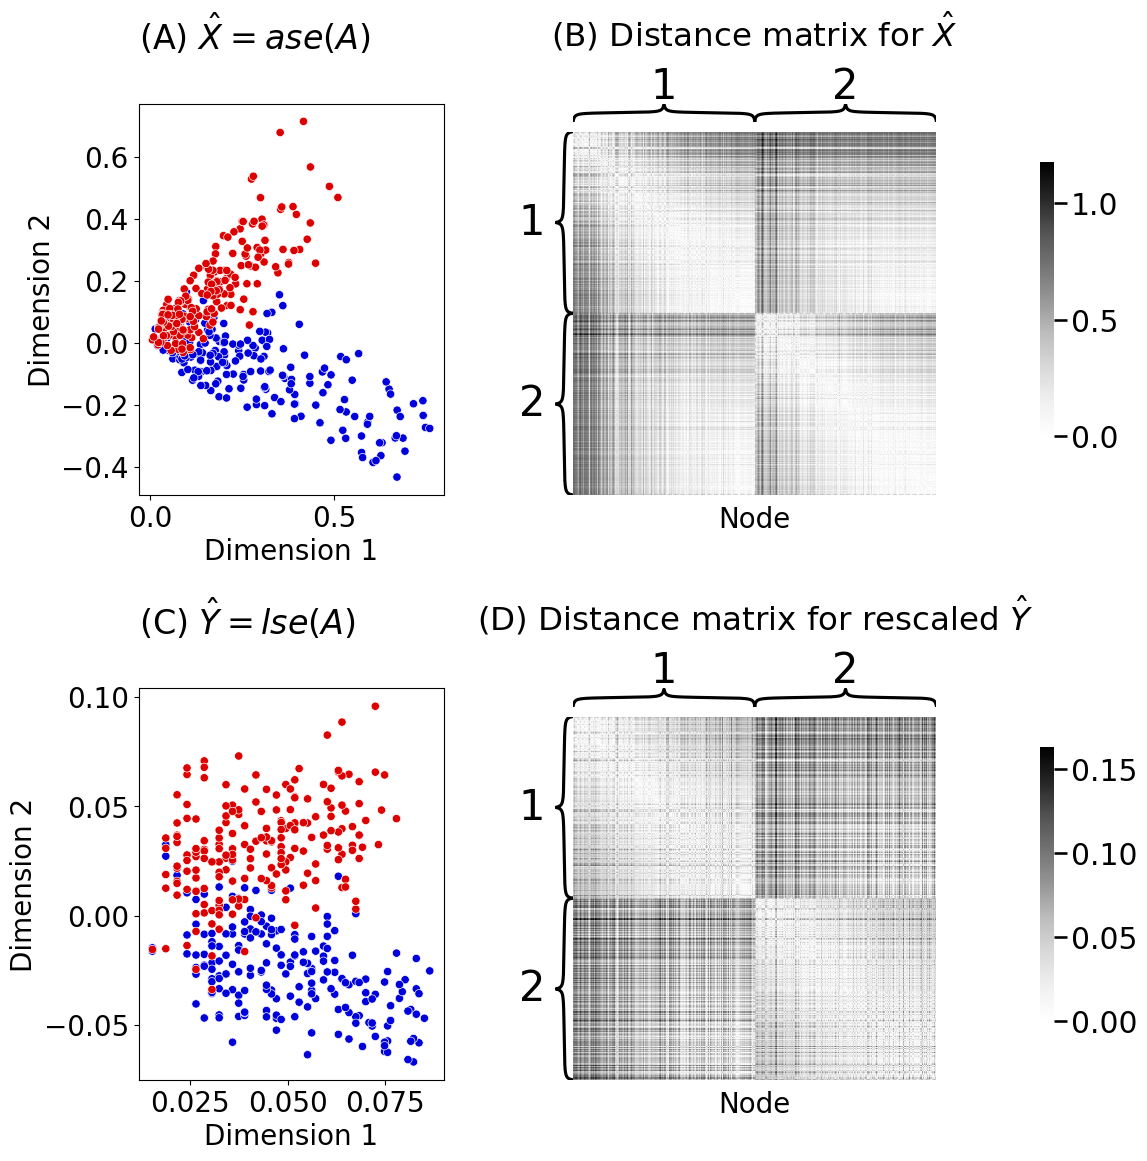
\includegraphics[width=\linewidth]{representations/ch6/Images/dcsbm_lse.png}
    \caption[LSE vs ASE, heavy-tailed example]{\textbf{(A)} the estimated latent positions, \textbf{(B)} the pairwise distances of estimated latent positions, \textbf{(C)} the estimated latent positions from \texttt{lse}, \textbf{(D)} the pairwise distances of the estimated latent positions from \texttt{lse}.}
    \label{fig:ch6:lse:dcsbm_lse}
\end{figure}

\subsection{Why do we use \texttt{lse}?}

The reasons to use \texttt{lse} are very similar to the reasons to use \texttt{ase}, which we explored in Section \ref{sec:ch6:ase:whyuse}. 

\subsubsection{When do we use \texttt{lse} over \texttt{ase}, and vice-versa?}

The primary difference between \texttt{lse} and \texttt{ase} is illustrated by example in Figure \ref{fig:ch6:lse:dcsbm_lse}. \texttt{ase} will capture estimates of latent positions, whereas \texttt{lse} will capture estimates of latent positions of the population network laplacian. Loosely, this has the consequence that \texttt{lse} will produce ``scaled'' estimates of latent positions that have been adjusted for degree differences in the underlying network. 

Often, we will want to learn about latent structures that are not related to the degrees of the nodes in the network. In such cases, these scaled estimates produced by \texttt{lse} will often make latent structure that we might want to find more obvious both visually (in heatmaps and pairs plots) and algorithmically (through the use of downstream models to identify latent structure from your estimated latent positions). 

A primary visualization to determine whether \texttt{ase} or \texttt{lse} are appropriate is to look at the {node degree histogram}. The node degree histogram is a histogram of the degrees for each node in the network. We can do this by first computing the node degrees in the network, and then plotting them as a histogram, using the insights that we build in Section \ref{sec:ch4:prop-net:degree}. Let's investigate this for the $DCSBM_n(\vec z, \vec \theta, B)$ sample we generated above:

\begin{lstlisting}[style=python]
import seaborn as sns

# compute the degrees for each node, using the
# row-sums of the network
degrees = A.sum(axis = 0)

# plot the degree histogram

df = pd.DataFrame({"Node degree" : degrees, "Community": z})
sns.histplot(data=df, x="Node degree", bins=20, color="black", hue="Community")
\end{lstlisting}

The key feature that we look for is whether the degree histogram is \textit{right-skewed} or \textit{heavy tailed}. Remember from Section \ref{sec:ch4:regularization:logscale} that a distribution is right-skewed if it ``tails off'' towards the relatively large values in the positive direction. In these situations, the node degrees are lower-bounded by zero (the networks are simple, so all the adjacencies $a_{ij}$ are either $0$ or $1$, and the node degrees are sums of adjacencies), so this is generally just referred to as a ``heavy tailed degree distribution'', since it can only ``tail off'' to the right (since it is bounded to the left by $0$). Note that in Figure \ref{fig:ch6:lse:degree}(A), the degree distribution for nodes across both communities tails off to the right. For $DCSBM_n(\vec z, \vec \theta, B)$ random networks where the degree-correction factors $\theta_i$ tend to have mostly relatively small values, but some relatively large values, that the degree is lower-bounded by $0$ will tend to yield heavy tailed degree distributions. 

This contrasts from $SBM_n(\vec z, B)$ random networks and $DCSBM_n(\vec z, \vec \theta, B)$ random networks where the degree-correction factor $\theta_i$ is constant for all nodes in the same community, which will tend to have symmetric degree distributions for each community.

\begin{lstlisting}[style=python]
Asbm = sbm([nk, nk], B)

# row-sums of the network
degrees_sbm = Asbm.sum(axis = 0)
\end{lstlisting}

The histogram for an $SBM_n(\vec z, B)$ random network is shown in Figure \ref{fig:ch6:lse:degree}(B). Note that the degree histogram appears to have two ``peaks'', and neither peak is particularly heavy tailed (they both look fairly mirrored). This plot provides evidence that the degree-distribution is not heavy tailed.

\begin{figure}[h]
    \centering
    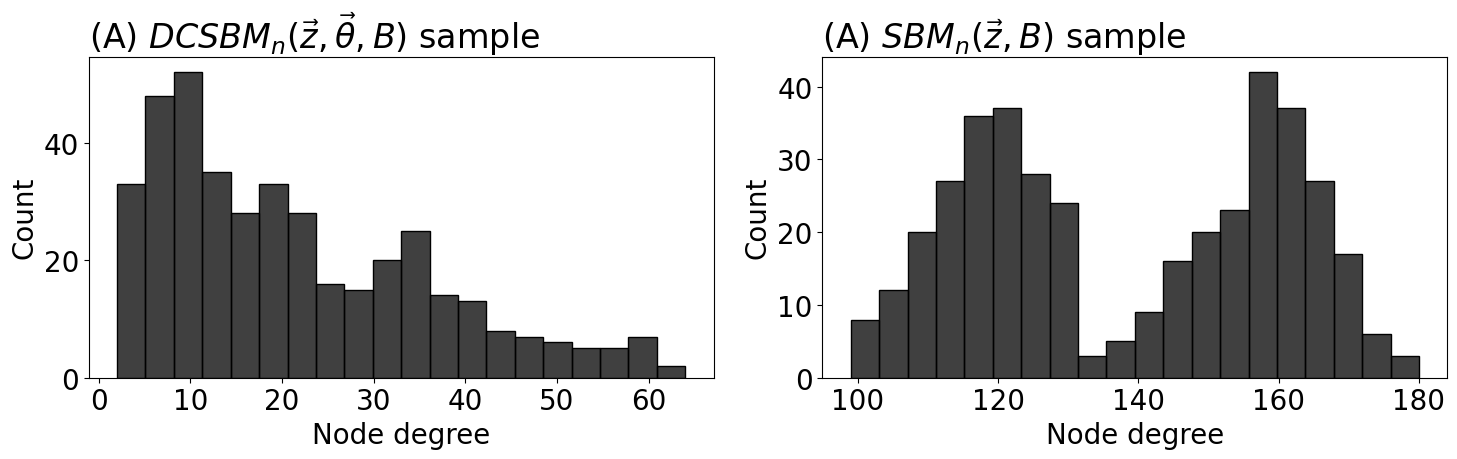
\includegraphics[width=\linewidth]{representations/ch6/Images/lse_degree.png}
    \caption[degree histogram for $DCSBM_n(\vec z, \vec \theta, B)$]{\textbf{(A)} the degree histogram for a $DCSBM_n(\vec z, \vec \theta, B)$ network, where the degree-correction factors are not equal for the nodes in the network. \textbf{(B)}the degree histogram for a $SBM_n(\vec z, B)$ network.}
    \label{fig:ch6:lse:degree}
\end{figure}

Heavy-tailed degree distributions frequently arise in real data \cite{Qin2013Sep, Muldoon2016Feb, Prakash2010}. This pattern is particularly apparent in networks that share features of core-periphery networks from Section \ref{sec:ch5:psd_block}, where a selection of nodes (the \textit{core}) have much higher node degrees than the nodes outside of the core (the \textit{periphery}) \cite{Prakash2010}. This pattern can materialize concurrently with other patterns, such as the example that we saw above with a $DCSBM_n(\vec z, \vec \theta, B)$ network with heterogeneous $\theta_i$s and homophilic networks. 

When you can identify a heavy-tailed degree distribution from visualizations such as the node degree histogram, \texttt{lse} may be advantageous to use over \texttt{ase}. This might assist you in uncovering latent structure in the estimates of latent positions that you use downstream in your analysis.

\begin{comment}
\section{Expected values and random networks}

\subsection{Expected values and the adjacency matrix}
Back in Section \ref{sec:ch4:prop-net:degree}, you learned about the degree matrix. To obtain the degree matrix, we started by computing the node degrees, where:
\begin{align*}
    d_i = \sum_{j = 1}^n a_{ij}
\end{align*}

Once we computed the node degrees, the degree matrix was the diagonal matrix where:
\begin{align*}
    D &= \begin{bmatrix}
        d_1 & & \\
        & \ddots & \\
        & & d_n
    \end{bmatrix},
\end{align*}

To understand the expected node degree, it is important to first clarify the expected outcome at a particular edge. We'll do this with as little statistics knowledge as possible. If $\mathbf x$ is a random quantity that takes one of two possible outcomes ($0$ or $1$), then the expected value is:
\begin{align*}
    \mathbb E[\mathbf x] = 1 Pr (\mathbf x = 1) + 0 Pr(\mathbf x = 0),
\end{align*}
where $Pr(\mathbf x = k)$ is just the probability that the random quantity $\mathbf x$ takes the value $k$. This is a very simple case of a statistical result that is commonly known as the \textit{Law of the Unconscious Statistician} (LoTUS).

We have already seen an instance of a random quantity that takes one of two possible outcomes ($0$ or $1$) in our work: the adjacencies for a random network, $\mathbf a_{ij}$. Remember that for an adjacency $\mathbf a_{ij}$, that $\mathbf a_{ij}$ behaves like flipping a coin which lands on Heads (a value of $1$) with probability $p_{ij}$, or Tails (a value of $0$) with probability $1 - p_{ij}$. Therefore, the expected value of each adjacency $\mathbf a_{ij}$ is:
\begin{align*}
    \mathbb E[\mathbf a_{ij}] &= p_{ij}
\end{align*}

This logic extends directly to matrices. If $\mathbf X$ is a matrix, then its expected value is:
\begin{align*}
    \mathbb E[\mathbf X] &= \begin{bmatrix}
        \mathbb E[\mathbf x_{11}] & \hdots & \mathbb E[\mathbf x_{1n}] \\
        \vdots & \ddots & \vdots \\
        \mathbb E[\mathbf x_{n1}] & \hdots & \mathbb E[\mathbf x_{nn}]
    \end{bmatrix}
\end{align*}
So, the expected value of a matrix is the matrix of expected values of each entry.

This has an important implication for our purposes. If $\mathbf A$ is an $IER_n(P)$ random network, then:
\begin{align*}
    \mathbb E[\mathbf A] = P
\end{align*}

Now, for our purposes, this is a little bit obtuse: we see samples $A$, not the random network $\mathbf A$, in practice.

As it turns out, there is another result that can help us here. If $\mathbf x$ and $\mathbf y$ are two finite random variables (which they always will be, in our case), then the expectation of the sum is the sum of the expectations. In words, we can write this down as:
\begin{align*}
    \mathbb E[\mathbf x + \mathbf y] = \mathbb E[\mathbf x] + \mathbb E[\mathbf y].
\end{align*}

Let's extend this to the case of taking an sum. Remember that a sum of $M$ numbers $x^{(m)}$ is defined as:
\begin{align*}
    \sum_{m = 1}^M x^{(m)}
\end{align*}
If we instead had $M$ random numbers $\mathbf x^{(m)}$, when we compute the expected value of the sum, it is the sum of the expected values:
\begin{align*}
   \mathbb E\left[\sum_{m = 1}^M x^{(m)}\right] &= \sum_{m = 1}^M \mathbb E\left[\mathbf x^{(m)}\right]
\end{align*}

So, let's imagine that we have $M$ adjacency matrices $\mathbf A^{(m)}$ that are each independent $IER_n(P)$ random networks with the same probability matrix. The expected average adjacency matrix would be:
\begin{align*}
    \mathbb E\left[\frac{1}{M}\sum_{m = 1}^M \mathbf A^{(m)}\right] &= 
\end{align*}
\end{comment}




\newpage